\documentclass[aspectratio=169]{beamer}

\mode<presentation>
{
  \usetheme{default}
  \usecolortheme{default}
  \usefonttheme{default}
  \setbeamertemplate{navigation symbols}{}
  \setbeamertemplate{caption}[numbered]
  \setbeamertemplate{footline}[frame number]  % or "page number"
  \setbeamercolor{frametitle}{fg=white}
  \setbeamercolor{footline}{fg=black}
} 

\usepackage[english]{babel}
\usepackage[utf8x]{inputenc}
\usepackage{tikz}
\usepackage{courier}
\usepackage{array}
\usepackage{bold-extra}
\usepackage{minted}
\usepackage[thicklines]{cancel}

\xdefinecolor{dianablue}{rgb}{0.18,0.24,0.31}
\xdefinecolor{darkblue}{rgb}{0.1,0.1,0.7}
\xdefinecolor{darkgreen}{rgb}{0,0.5,0}
\xdefinecolor{darkgrey}{rgb}{0.35,0.35,0.35}
\xdefinecolor{darkorange}{rgb}{0.8,0.5,0}
\xdefinecolor{darkred}{rgb}{0.7,0,0}
\definecolor{darkgreen}{rgb}{0,0.6,0}
\definecolor{mauve}{rgb}{0.58,0,0.82}

\title[2018-06-04-scipyeco-hats]{Scientific Python Ecosystem HATS}
\author{Jim Pivarski}
\institute{Princeton University -- DIANA-HEP}
\date{June 4, 2018}

\begin{document}

\logo{\pgfputat{\pgfxy(0.11, 7.4)}{\pgfbox[right,base]{\tikz{\filldraw[fill=dianablue, draw=none] (0 cm, 0 cm) rectangle (50 cm, 1 cm);}\mbox{\hspace{-8 cm}
\includegraphics[height=1 cm]{princeton-logo-long.png}
\includegraphics[height=1 cm]{diana-hep-logo-long.png}}}}}

\begin{frame}
  \titlepage
\end{frame}

\logo{\pgfputat{\pgfxy(0.11, 7.4)}{\pgfbox[right,base]{\tikz{\filldraw[fill=dianablue, draw=none] (0 cm, 0 cm) rectangle (50 cm, 1 cm);}\mbox{\hspace{-8 cm}
\includegraphics[height=1 cm]{princeton-logo.png}
\includegraphics[height=1 cm]{diana-hep-logo.png}}}}}

% Uncomment these lines for an automatically generated outline.
%\begin{frame}{Outline}
%  \tableofcontents
%\end{frame}

% START START START START START START START START START START START START START

\begin{frame}{}
\begin{center}
\LARGE \textcolor{darkblue}{Big data: we're not the only ones doing it}
\end{center}
\end{frame}

\begin{frame}{{200~PB is a lot of data}\only<2>{, but for Amazon, it's two trucks}}
\vspace{0.35 cm}
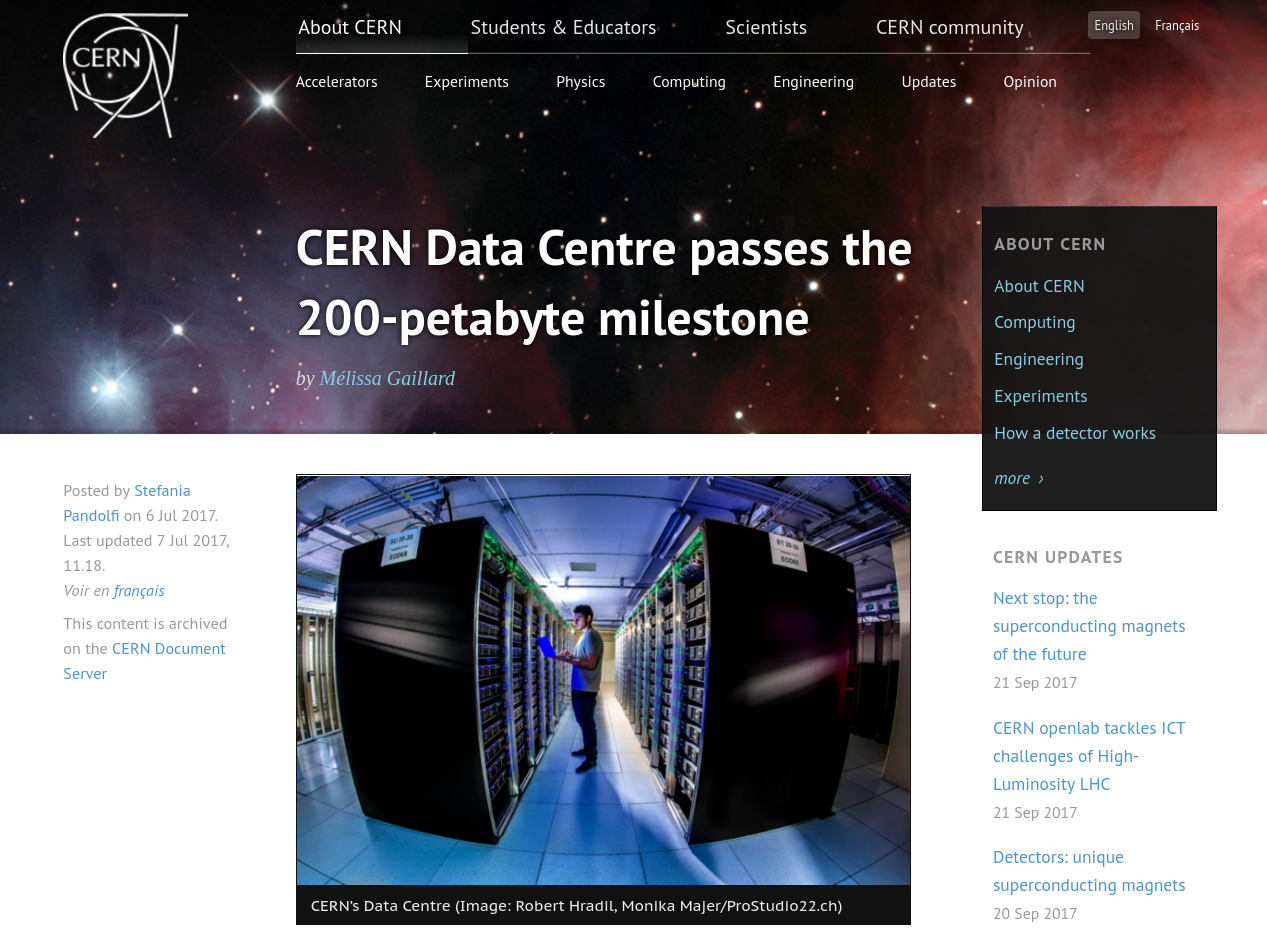
\includegraphics[width=0.73\linewidth]{cern-200pb.png}

\vspace{-4.8 cm}
\uncover<2->{\mbox{ } \hfill 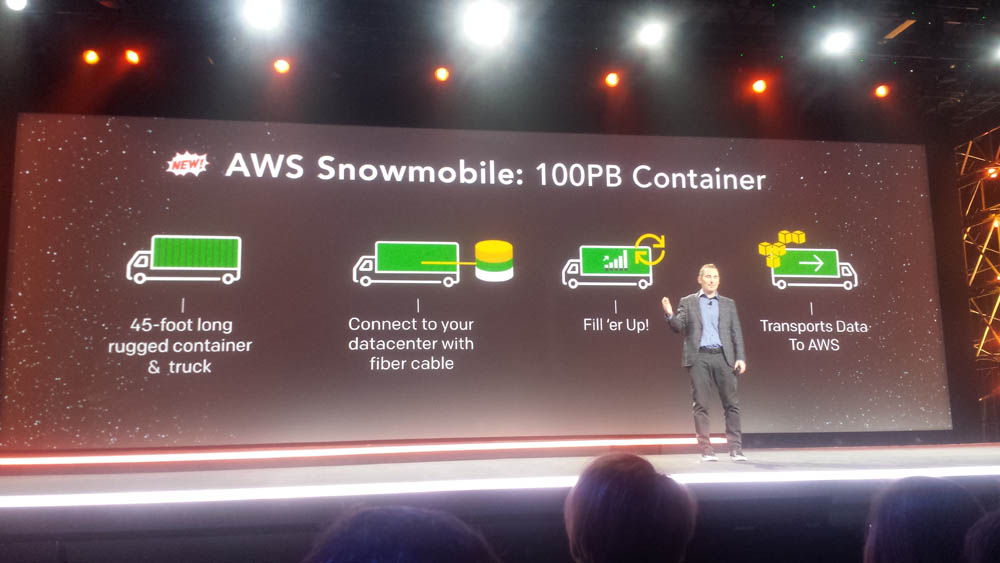
\includegraphics[width=0.7\linewidth]{aws-snowmobile.jpg}\hspace{-1 cm}}
\end{frame}

\begin{frame}{Data analysis software developed independently on both sides}
\vspace{0.17 cm}
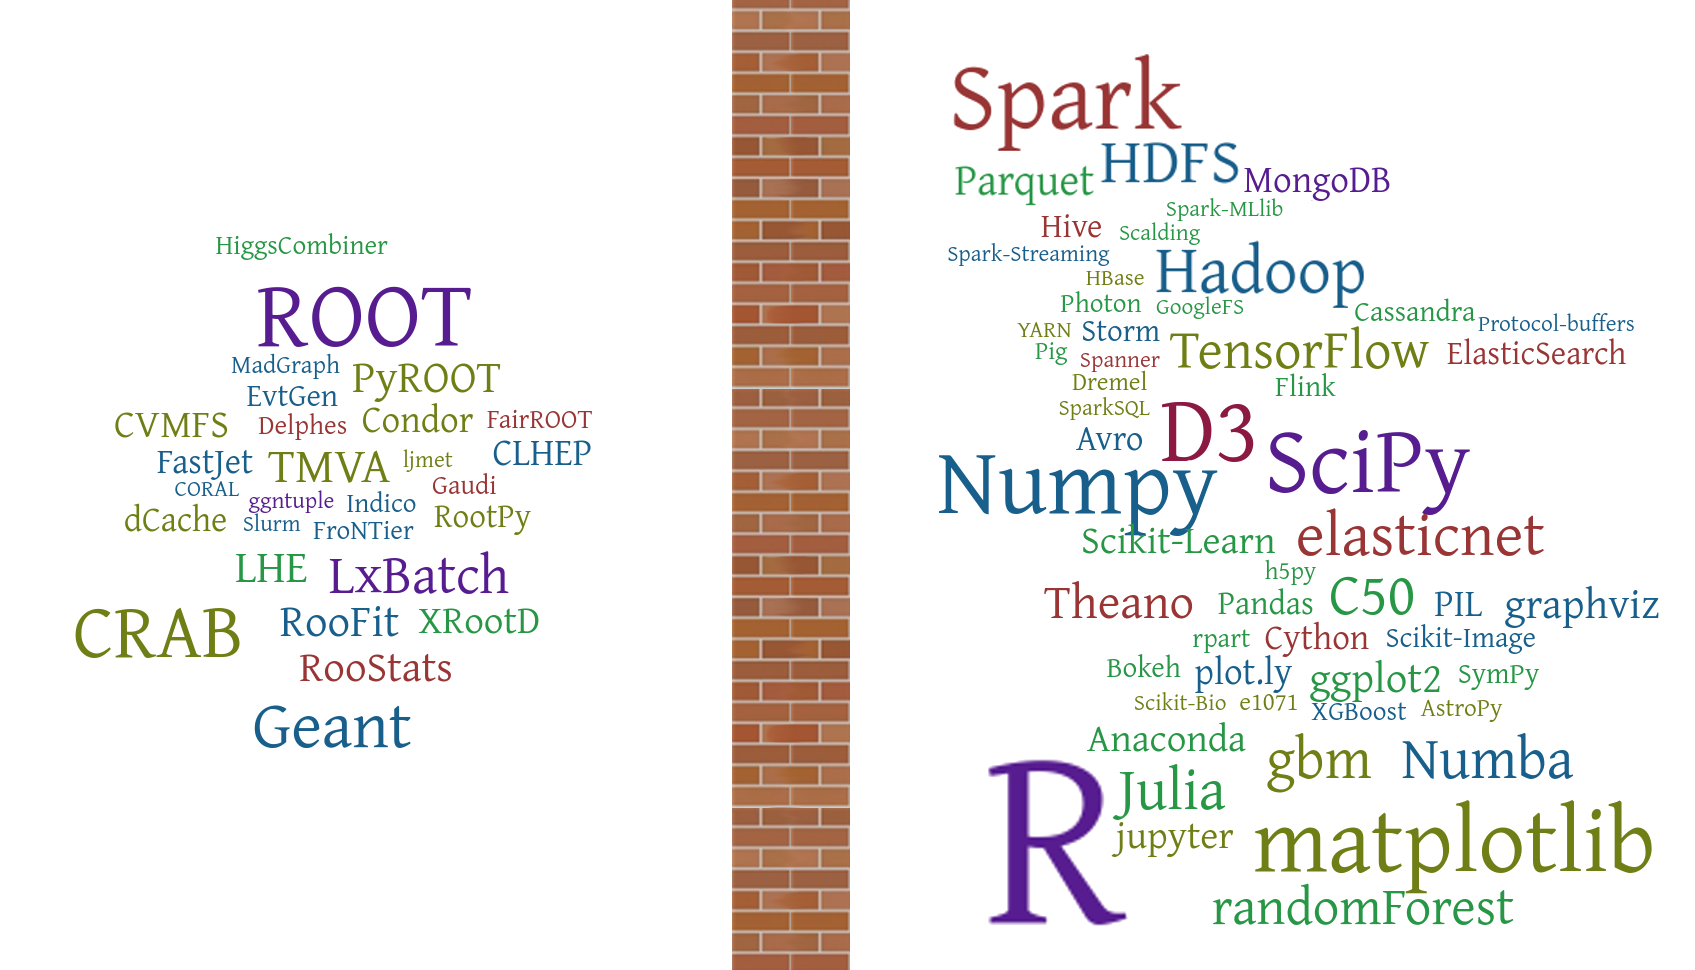
\includegraphics[width=\linewidth]{separation-2.png}
\end{frame}

\begin{frame}{Python is emerging as a favorite language for data analysis}
\vspace{0.5 cm}
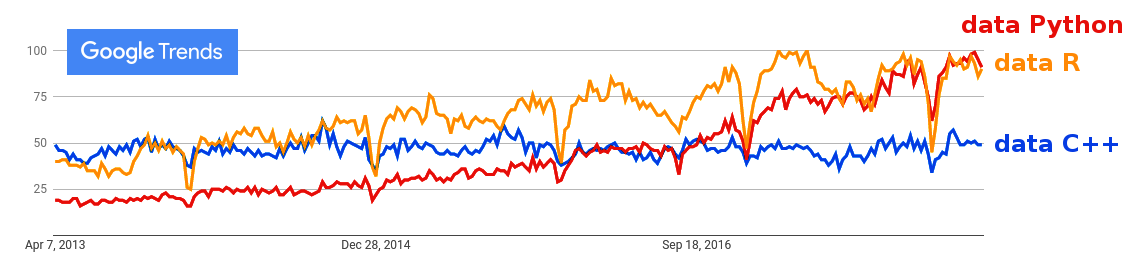
\includegraphics[width=\linewidth]{python-r-cpp-googletrends-data.png}

\vspace{1 cm}
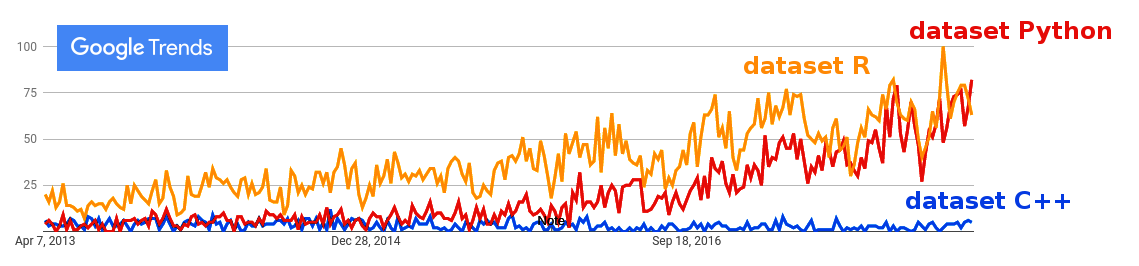
\includegraphics[width=\linewidth]{python-r-cpp-googletrends-dataset.png}
\end{frame}

\begin{frame}{Python is emerging as a favorite language for data analysis}
\vspace{0.5 cm}
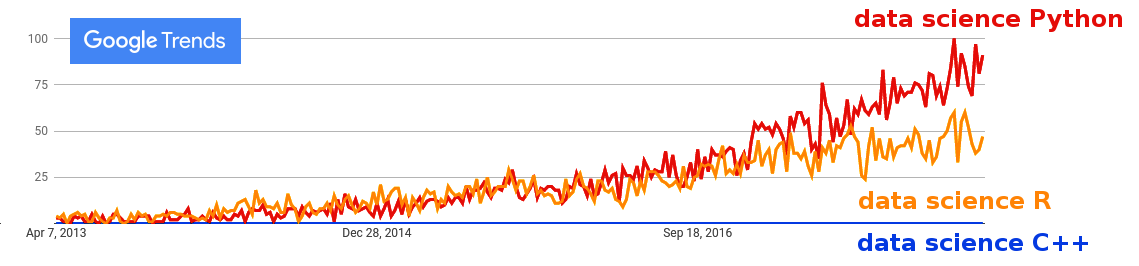
\includegraphics[width=\linewidth]{python-r-cpp-googletrends-datascience.png}

\vspace{1 cm}
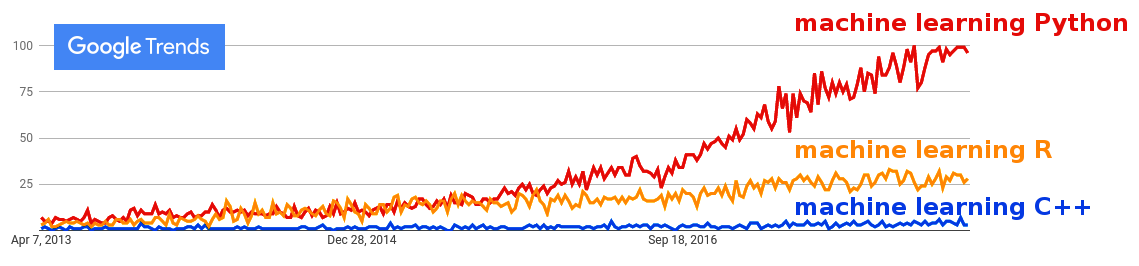
\includegraphics[width=\linewidth]{python-r-cpp-googletrends-machinelearning.png}
\end{frame}

\begin{frame}{Scientific Python ecosystem}
\vspace{0.35 cm}
\textcolor{darkblue}{The word ``ecosystem'' is deliberately vague: no clear boundaries, but a few key components and many projects that share conventions.}

\begin{columns}
\column{1.1\linewidth}
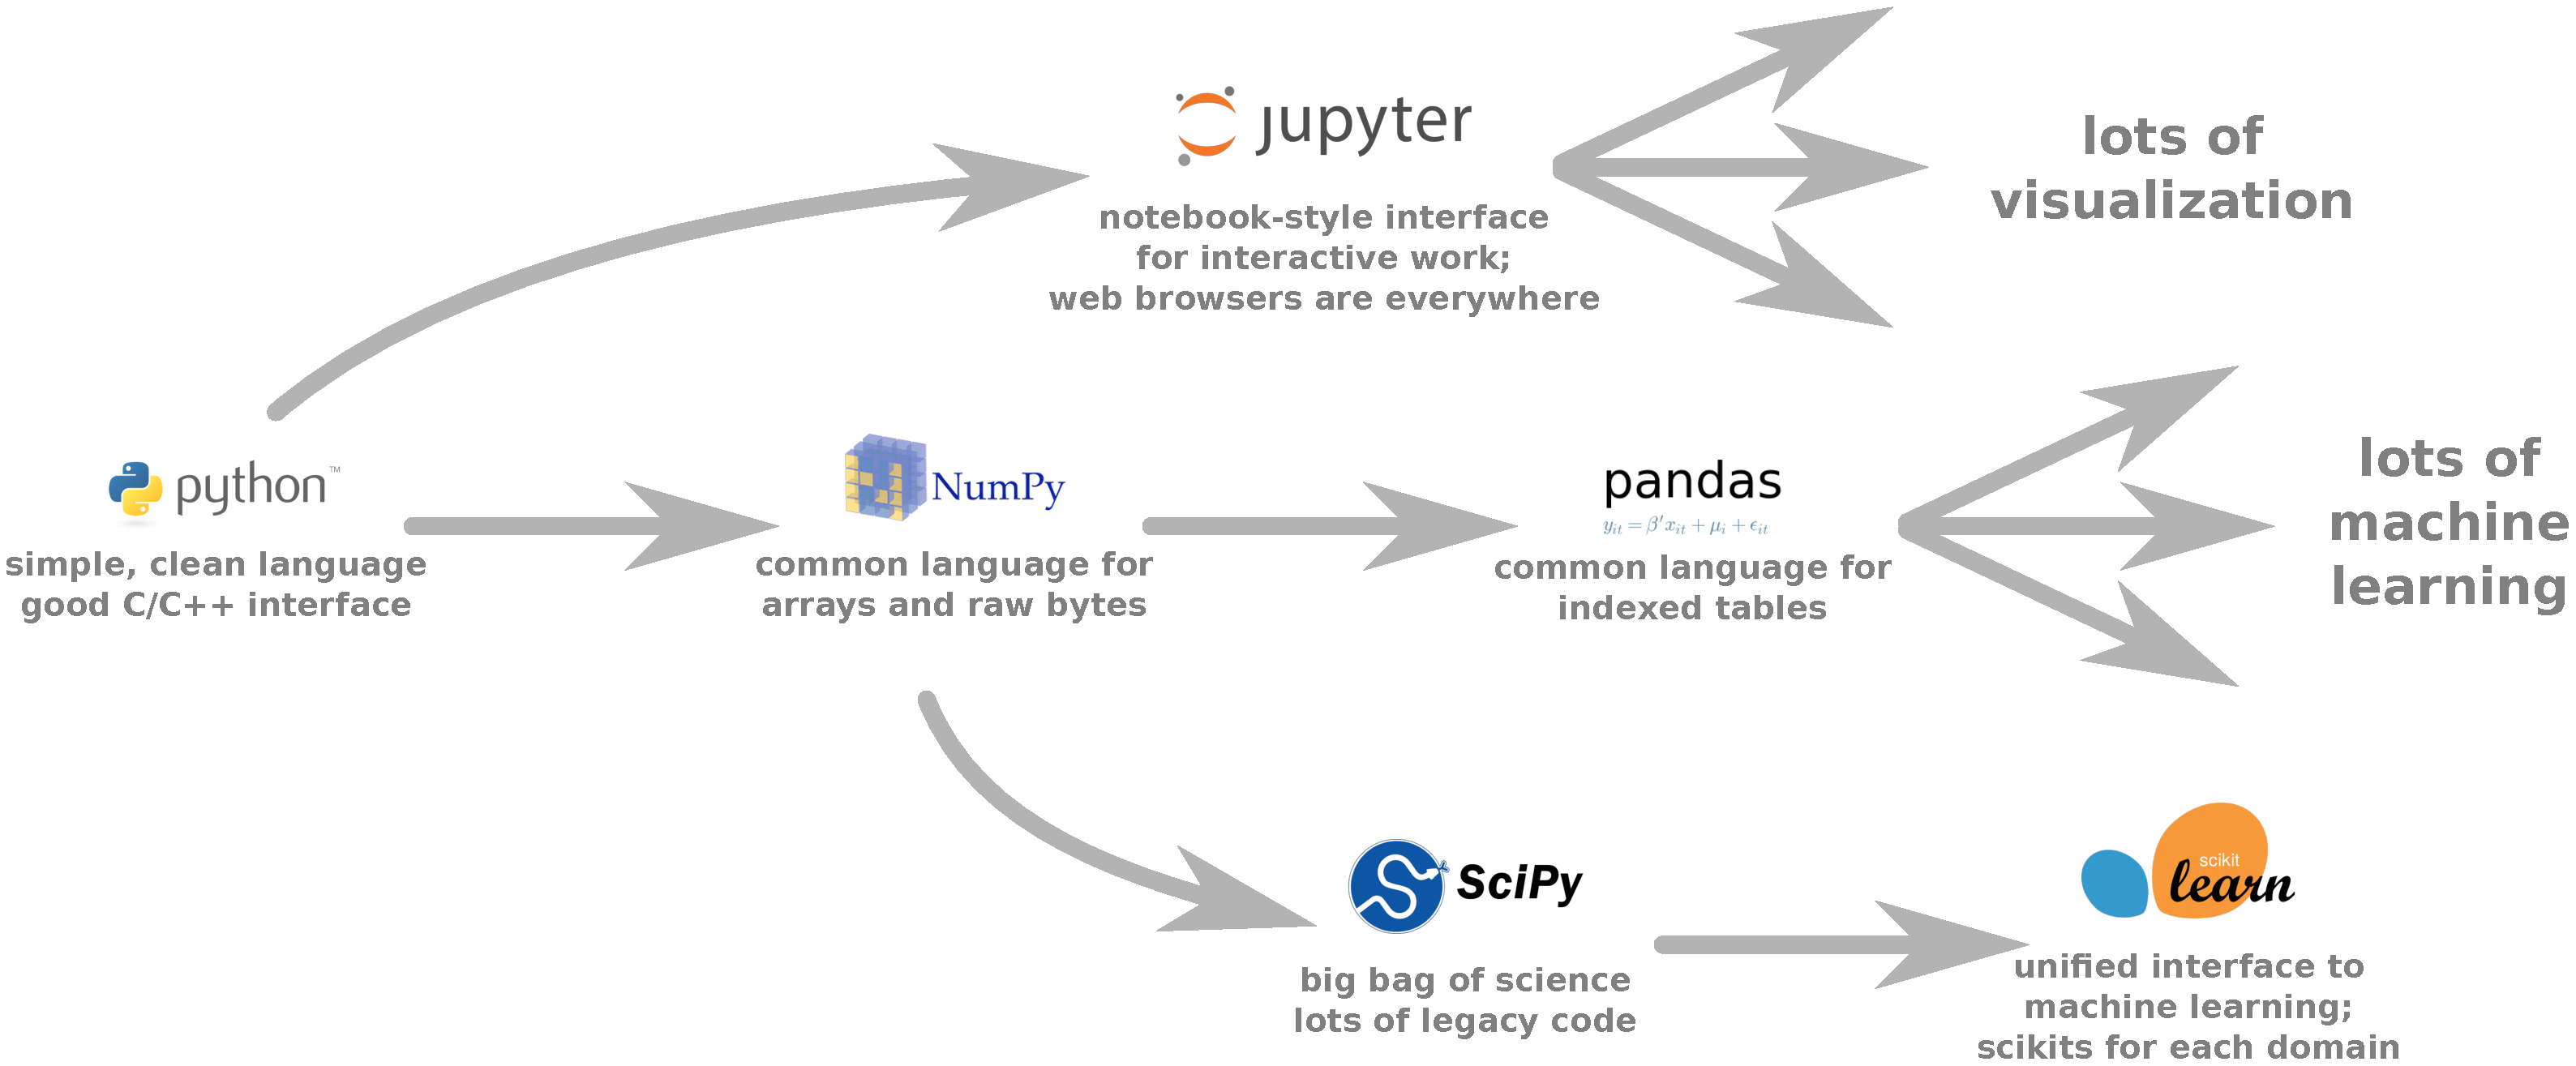
\includegraphics[width=\linewidth]{software-ecosystem.pdf}
\end{columns}
\end{frame}

\begin{frame}[fragile]{Python the language and CPython the implementation}
\vspace{0.5 cm}
\hfill 
\includegraphics[height=1 cm]{python-logo.png}

\vspace{-1 cm}
\textcolor{darkblue}{Exercise:} open a Python session {\scriptsize (you all have one, except maybe Windows)}

\small
\begin{minted}{python}
>>> import antigravity
\end{minted}
\normalsize

and see what happens\ldots

\vspace{0.5 cm}
\begin{uncoverenv}<2->
Like \LaTeX, the microsyntax is extremely usable: easy to get started on small things.

(Also like \LaTeX, large programs are awkward.)
\end{uncoverenv}

\vspace{0.5 cm}
\begin{uncoverenv}<3->
Unlike Java, one implementation (CPython) is much more popular than the others (PyPy, Jython, IronPython, CLPython\ldots), with good bindings to C/C++.
\end{uncoverenv}

\vspace{0.5 cm}
\begin{uncoverenv}<4->
\small
\textcolor{darkblue}{Questions (show of hands):}
\vspace{-0.2 cm}
\begin{enumerate}\setlength{\itemsep}{-0.1 cm}
\item How many people have used Python a lot?
\item A little?
\item Not at all?
\end{enumerate}
\end{uncoverenv}
\end{frame}

\begin{frame}{Numpy arrays}
\vspace{0.5 cm}
\hfill 
\includegraphics[height=1.3 cm]{numpy-logo.png}

\vspace{-1.3 cm}

Python is high-level, not designed for numeric processing.

Numpy is the key that made scientific data analysis possible.

\vspace{0.25 cm}
\begin{uncoverenv}<2->
\textcolor{darkblue}{Bad old days:} numarray for large arrays, Numeric for small ones $\to$ Numpy in 2005.
\end{uncoverenv}

\vspace{0.25 cm}
\begin{uncoverenv}<3->
``Vectorized'' calculations: instead of doing a lot of operations on one event before moving on to the next, do one operation across a batch of events, then the next, etc., to avoid stepping through slow Python (we'll see examples).
\end{uncoverenv}

\vspace{0.25 cm}
\begin{uncoverenv}<4->
Very similar to vectorization for GPUs and new CPUs: new hardware can apply the same instruction to multiple values at once. I think it's a historical irony that the same technique to speed up a high-level language is now speeding up bare metal.
\end{uncoverenv}

\vspace{0.25 cm}
\begin{uncoverenv}<5->
\small
\textcolor{darkblue}{Questions (show of hands):}
\vspace{-0.2 cm}
\begin{enumerate}\setlength{\itemsep}{-0.1 cm}
\item How many people have performed vectorized calculations in Numpy?
\item How many have used it at all?
\item How many haven't?
\end{enumerate}
\end{uncoverenv}
\end{frame}

\begin{frame}{Pandas data frames}
\vspace{0.35 cm}
\hfill 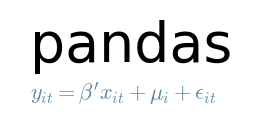
\includegraphics[height=1.3 cm]{pandas-logo.png}

\vspace{-1.3 cm}
Numpy provides in-memory data tables with slick indexing.

\vspace{0.05 cm}
\uncover<2->{Pandas provides in-memory data tables with slick indexing.}

\vspace{0.05 cm}
\uncover<3->{Pandas is considered an enabling technology for data science.}

\vspace{0.35 cm}
\uncover<4->{\textcolor{darkblue}{What's the big deal?}}

\begin{itemize}\setlength{\itemsep}{0.1 cm}
\item<5-> The rows of Pandas data frames are indexed: each row {\it means} something.

\vspace{0.1 cm}
\uncover<6->{For example, adding two data frames with different sets of keys matches the overlapping sets of keys and unions the others, more like a {\tt\small dict} than a {\tt\small list}.}

\vspace{0.1 cm}
\uncover<7->{Think ``systematics studies,'' not ``bag of events.''}

\item<8-> Includes built-in plotting and statistics.

\item<9-> Common target for user-oriented statistical packages, especially machine learning.
\end{itemize}

\vspace{0.35 cm}
\begin{uncoverenv}<10->
\small
\textcolor{darkblue}{Questions (show of hands):}
\vspace{-0.2 cm}
\begin{enumerate}\setlength{\itemsep}{-0.1 cm}
\item How many people have used Pandas?
\item How many haven't?
\end{enumerate}
\end{uncoverenv}
\end{frame}

\begin{frame}{SciPy libraries}
\vspace{0.25 cm}
\hfill 
\includegraphics[height=1 cm]{scipy-logo.png}

\vspace{-1 cm}

\vfill
\small
\textcolor{darkblue}{Questions (show of hands):}
\vspace{-0.2 cm}
\begin{enumerate}\setlength{\itemsep}{-0.1 cm}
\item How many people have used at least one function from SciPy?
\item How many haven't?
\end{enumerate}
\end{frame}

\begin{frame}{Jupyter notebooks}
\vspace{0.25 cm}
\hfill 
\includegraphics[height=0.8 cm]{jupyter-logo.png}

\vspace{-0.8 cm}

\vfill
\small
\textcolor{darkblue}{Questions (show of hands):}
\vspace{-0.2 cm}
\begin{enumerate}\setlength{\itemsep}{-0.1 cm}
\item Is this your first time using Jupyter?
\item Do you plan on using it for normal work?
\end{enumerate}
\end{frame}

\begin{frame}{Scikit-Learn and other machine learning tools}
\vspace{0.25 cm}
\hfill 
\includegraphics[height=1.1 cm]{sklearn-logo.png}

\vspace{-1.1 cm}

\vfill
\small
\textcolor{darkblue}{Questions (show of hands):}
\vspace{-0.2 cm}
\begin{enumerate}\setlength{\itemsep}{-0.1 cm}
\item Who has used a machine learning package in Python (not TMVA)?
\item Who has used TMVA (in ROOT, possibly through PyROOT)?
\item Who hasn't?
\end{enumerate}
\end{frame}

\begin{frame}{What makes software ``Pythonic?''}
\end{frame}

\end{document}
